\documentclass{article}
\usepackage{graphicx} % Required for inserting images
\usepackage{amsmath, amssymb, amsthm}
\usepackage{algorithm}
\usepackage{algpseudocode}
\usepackage{amsmath, amssymb, amsthm}
\usepackage{float, fullpage, graphicx, multirow,parskip, subcaption, setspace}
\usepackage{comment}
\usepackage{url}
\usepackage{enumitem}
\usepackage{tikz}
\usepackage{bm, bbm}
\usepackage{booktabs}
\usepackage{caption}
\usetikzlibrary{shapes.geometric, positioning}
\usetikzlibrary{quotes, angles}
\usepackage{rotating}
\usepackage{hyperref}
\usepackage{natbib}

\title{Advanced MCMC Final Project}
\author{Christian Paul Ryan Morgan }
\date{September 2024}

\begin{document}

\maketitle

\section{Model Selection} 
Design and implement an algorithm that returns samples of $(S, \beta(S))$. Explicitly describe the cross-model moves (i.e., those that move between $(S, \beta(S))$ and $(S', \beta(S'))$ where $S, S'$ are distinct subsets of $\{1, 2, \dots, p\}$). \\ 


In this problem, we have $p$ covariates, $X_1, \ldots, X_p$, and an outcome $Y$. We have $2^p$ possible regression models, one for each subset $S$ of covariates, and each has its own parameter $\beta^{(S)}$. We wish to perform inference on $(S, \beta^{(S)})$.

We specify a uniform prior on $S$, so that $p(S) = 2^{-p}$ for all subsets.

Below, we describe an algorithm that returns samples of $(S, \beta^{(S)})$.

Let's first generate a Uniform random variable $R$ from [0,1] to determine what type of move we would like.

Now, we describe the model moves. There are 4 possible types of moves. 

The first possible move is a "stay" move. In this move, we let $(S, \beta) \to (S, \beta')$. We will perform a standard Metropolis-Hasting move here, and let $\beta' \sim N_{|S|}(0, I_{|S|})$. We perform this move if $R \in [0, .25)$.

The second possible move is a cross model move, called "add". Here, $(S, \beta) \to (S', \beta')$, where $|S'| = |S|+1$. Let $U \sim Unif[0,1]$. Then let $h(\beta_1, U) = (\beta_1, \beta_2)$. We perform this move if $R \in [.25, .5)$.

The third possible move is "delete". Let $(S, \beta) \to (S', \beta')$, where $|S'| = |S| - 1$. Let $h(\beta_1, \beta_2) = (\beta_1, U)$. We perform this move if $R \in [0.5, .75)$.

The last type of move is "swap". Again, $(S, \beta) \to (S', \beta')$, with $|S'| = |S|$. We let $h(\beta^S) = (\beta^{S'})$. We perform this move if $R \in [.75, 1]$.


Below, we report table indicating the results of running the algorithm above for 50,000 iterations with $p=5$ and $p=10$ variables.

\begin{table}[H]
    \centering
  \caption{Counts and posterior model probabilities for various sets when $p = 5$. The true set is the one with only X3, X4, and X5.}
  \begin{tabular}{| l c  c  c  c  c c |}
  \hline
  X1 & X2 & X3 & X4 & X5 & n & p \\
  \hline
FALSE  & FALSE  & TRUE  & TRUE  & TRUE  & 36416  & 0.728  \\
TRUE  & FALSE  & TRUE  & TRUE  & TRUE  & 6111  & 0.122  \\
FALSE  & TRUE  & TRUE  & TRUE  & TRUE  & 4949  & 0.099  \\
TRUE  & TRUE  & TRUE  & TRUE  & TRUE  & 2512  & 0.05  \\
FALSE  & FALSE  & FALSE  & TRUE  & TRUE  & 8  & 0  \\
TRUE  & FALSE  & FALSE  & FALSE  & TRUE  & 3  & 0  \\
FALSE  & FALSE  & FALSE  & FALSE  & TRUE  & 1  & 0  \\
\hline
\end{tabular}
\label{tab:prior_table_class}
\end{table}

The results of the simulations show that the algorithm returns samples that generally follow the true model, at least in terms of inclusion of the correct variables.

\begin{table}[H]
    \centering
  \caption{The top 8 counts and posterior model probabilities for various sets when $p = 10$. The true set is the one with only X3.}
  \begin{tabular}{| l c  c  c  c  c c c c c c c|}
  \hline
  X1 & X2 & X3 & X4 & X5 & X6 & X7 & X8 & X9 & X10 & n & p \\
  \hline
FALSE  & FALSE  & TRUE  & FALSE  & FALSE  & FALSE  & FALSE  & FALSE  & FALSE  & FALSE  & 41218  & 0.824  \\
FALSE  & FALSE  & TRUE  & FALSE  & FALSE  & FALSE  & FALSE  & FALSE  & TRUE  & FALSE  & 1742  & 0.035  \\
FALSE  & FALSE  & TRUE  & FALSE  & TRUE  & FALSE  & FALSE  & FALSE  & FALSE  & FALSE  & 1159  & 0.023  \\
FALSE  & FALSE  & TRUE  & FALSE  & FALSE  & TRUE  & FALSE  & FALSE  & FALSE  & FALSE  & 819  & 0.016  \\
FALSE  & FALSE  & TRUE  & FALSE  & FALSE  & FALSE  & TRUE  & FALSE  & FALSE  & FALSE  & 756  & 0.015  \\
FALSE  & FALSE  & TRUE  & FALSE  & FALSE  & FALSE  & FALSE  & FALSE  & FALSE  & TRUE  & 662  & 0.013  \\
TRUE  & FALSE  & TRUE  & FALSE  & FALSE  & FALSE  & FALSE  & FALSE  & FALSE  & FALSE  & 596  & 0.012  \\
FALSE  & FALSE  & TRUE  & FALSE  & FALSE  & FALSE  & FALSE  & TRUE  & FALSE  & FALSE  & 547  & 0.011  \\
\hline
\end{tabular}
\end{table}



\section{MALA for Standard Normals}

How sample size grows as MCMC iterations increases \\
Examining the bias of estimating the first and second moments of the distribution, which are known in advance \\ 



Parameters: $\lambda, d, \theta \in\mathbb{R}^{d}$
\begin{align}
    & \theta_{k+1} = \theta_{k} + \frac{1}{2}\lambda^{2} \nabla log(\pi(\theta_{k}) 
\end{align}

We tested our the performance of our MALA sampler on a grid of values of dimension $d = 1, 10, 100$ and step sizes $\lambda = 0.25, 0.5, 1, 2$.
For each experiment, we used a burn-in period of 1000 iterations.
We ran experiments where we kept 1000 to 10000 iterations, incremented by 1000.
We evaluate the performance of our sampler using effective sample size (ESS) and the bias of the true mean and variance of the distribution.

We find that our MALA sampler is sensitive to both $d$ and $\lambda$.
Figure \ref{fig:mala_std_normal} provides a visualization of our results.
When $d = 1$, larger step sizes tend to lead to higher ESS and reduced bias.
However, as $d$ grows, smaller step sizes tend to lead to better sampling diagnostics.
In general, our sampler struggles to fully explore the sample space in high dimensions, even with favorable hyperparameter settings.

\begin{figure}
\centering
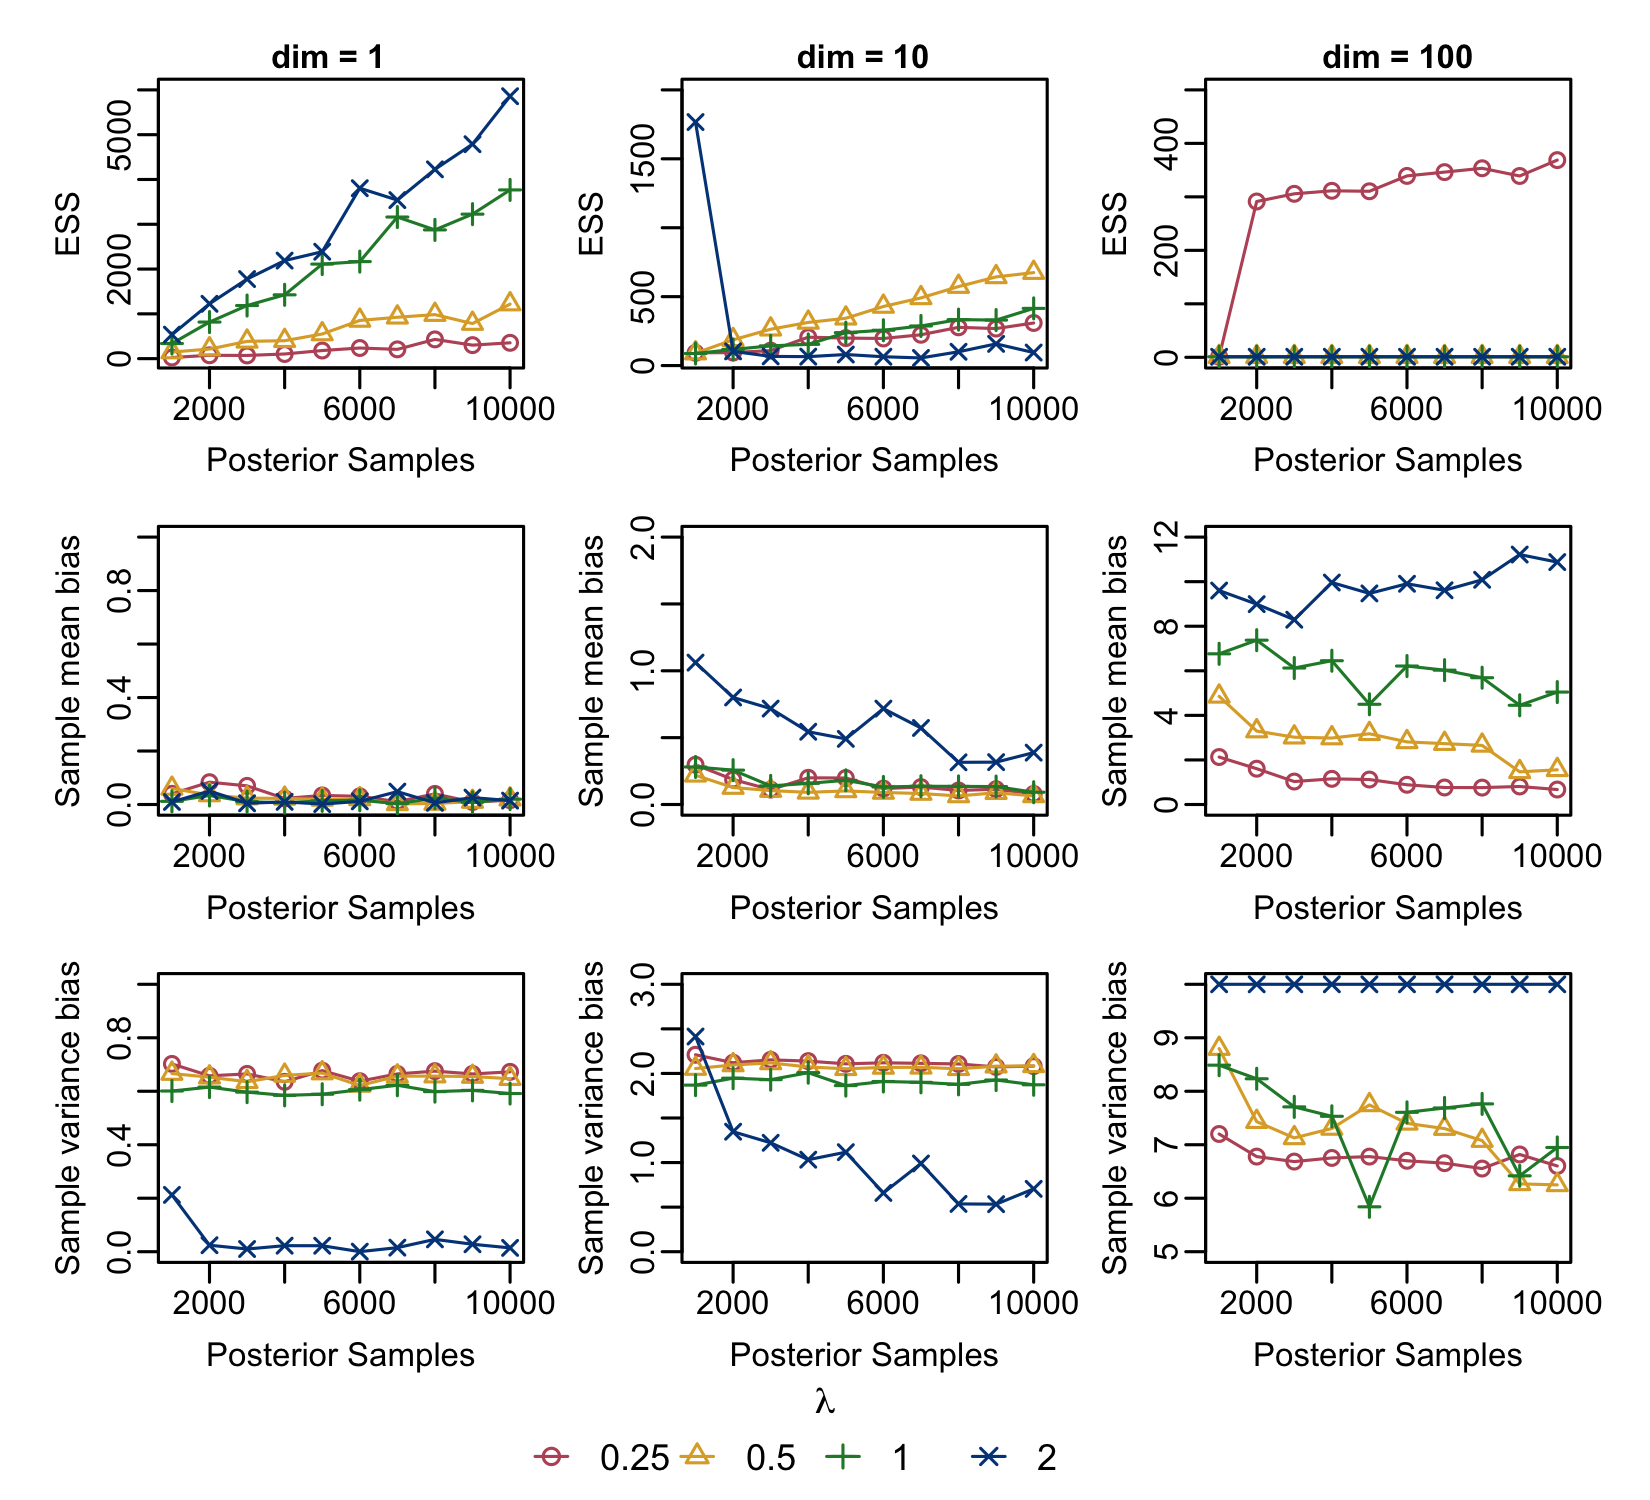
\includegraphics[width=.8\textwidth]{MALA_std_normal/mala_std_normal_diagnostics.png}
\caption{Diagnostics of standard normal MALA sampler experiments.}
\label{fig:mala_std_normal}
\end{figure}

\section{MALA for Bayesian Logistic Regression}

\subsection{Derivations}

We first derive the MALA iteration for Bayesian Logistic Regression. 
To do this, we derive two quantities: the gradient of the log of the target distribution, 
and the acceptance ratio when used in the metropolis-hasting framework.

\paragraph{Gradient Derivation.} 
The target distribution in our example is the posterior distribution of $\beta \in \mathbb{R}^p$, conditional
on observations $y_1,...,y_n \in \mathbb{R}$ following the model
\begin{align}
    y_i | \beta &\sim \text{Bern}(\left[ 1 + \exp(-x_i^\intercal \beta) \right]^{-1})\\
    \beta &\sim \mathcal{N}(0, I).
\end{align}
The resulting log posterior likelihood is (up to a constant term independent of $\beta$)
\begin{align} \label{p3-eq-log-posterior}
    \log ( p(\beta | y_1,...,y_n) ) &= \sum_{i=1}^n \log( p(y_i | \beta)) + \log(p(\beta))\\
    &= \left( 
        \sum_{i=1}^n -y_i \log(1+\exp(-x_i^\intercal \beta)) 
        + (1-y_i) \log\left( \frac{\exp(-x_i^\intercal\beta)}{1+\exp(-x_i^\intercal\beta)}\right) 
        \right) - .5 ||\beta||_2^2\\
    &= \sum_{i=1}^n -\log\left( 1+\exp(-x_i^\intercal\beta) \right) + (y_i-1)(x_i^\intercal \beta) - .5 ||\beta||_2^2. \\
\end{align} 
Taking the gradient of equation \ref{p3-eq-log-posterior} results in
\begin{equation}
    \nabla_{\beta} \log( p(\beta | y_1,...,y_n) ) = \sum_{i=1}^n \frac{1}{1 + \exp(x_i^\intercal\beta)} x_i + (y_i - 1) x_i.
\end{equation}

\paragraph{Acceptance Ratio Derivation.} 
To fully specify MALA, we must calculate the acceptance ratio; for $\beta$ and a proposed $\beta'$
\begin{equation} \label{p3-eq-acceptance-ratio}
    \alpha_3
    = \min\left\{1, \frac{p(\beta' | y_1,...,y_n) q(\beta | \beta')}{p(\beta | y_1,...,y_n) q(\beta' | \beta)} \right\} 
    = \min\left\{1, \frac{p(y_1,...,y_n | \beta')}{p(y_1,...,y_n | \beta)}\right\}.
\end{equation}
For numerical stability, we compute $\log(\alpha_3)$ in our algorithm.

\subsection{Results}
Having derived the gradient term and acceptance ratio in equations \ref{p3-eq-log-posterior} and \ref{p3-eq-acceptance-ratio}, 
we now present our numerical results.
Our experiment parameters are summarized below.
\begin{enumerate}
    \item We range the number parameters, $p$, in the set $\{1, 10, 100\}$.
    \item We range the number step size, $\lambda$, in the set $\{10^{-4}, 10^{-3}, 10^{-2}, 10^{-1}\}$.
    \item For each $p$, $n=1000$ points are samples from the model, and $20000$ MALA steps were generated with $5000$ discarded as a burn in. 
    For HMC, 4 chains were used, each taking $2000$ iterations. 
\end{enumerate}
We implement the code for MALA in julia. The results of the experiment for MALA are in Table \ref{table-results-mala}, and the results for HMC are in \ref{table-results-HMC}.
\begin{table}[ht]
    \centering
    \caption{Results for MALA. Going from left to right, the first table shows effective sample size, time (in seconds), and posterior bias ($||\beta_* - \hat{\beta}||_2^2$).}
    \label{table-results-mala}
    \footnotesize
    \begin{tabular}{| c | c c c || c c c || c c c |} \toprule
    Results MALA                    & & ESS &  &  & Time &  & & Posterior Bias &  \\ \midrule
    $\lambda / p$                    & $p=1$ & $p = 10$ & $p = 100$ & $p=1$ & $p = 10$ & $p = 100$ & $p=1$ & $p = 10$ & $p = 100$ \\ \midrule 
    $\lambda = 10^{-4}$   &  5.54     &    24.77      &     295.56      &   3.2   &   5.10    &    40.29  &     0.16     &    9.0      &  116.76 \\
    $\lambda = 10^{-3}$   &  5.52    &    41.83      &    324.29      &   1.9    &  5.12     &   42.15  &     0.02     &      3.75    & 87.1162\\
    $\lambda = 10^{-2}$   &  65.16     &  73.3       &    300.62       &   1.9    &  5.11     &   43.8   &     0.0003      &    0.25      & 8.16\\
    $\lambda = 10^{-1}$   &  4832.35    &  2020.81        &   710.28        &   1.9    &  5.43     &   43.9   &     0.0005      &    0.23      & 8.11 \\\bottomrule
    \end{tabular}
\end{table}

\begin{table}[!ht]
    \centering
    \caption{Results for HMS. Going from left to right, the first table shows effective sample size, time (in seconds), and posterior bias ($||\beta_* - \hat{\beta}||_2^2$).}
    \label{table-results-HMC}
    \footnotesize
    \begin{tabular}{| c | c c c || c c c || c c c |} \toprule
    Results HMC                    & & ESS &  &  & Time &  & & Posterior Bias &  \\ \midrule
       & $p=1$ & $p = 10$ & $p = 100$ & $p=1$ & $p = 10$ & $p = 100$ & $p=1$ & $p = 10$ & $p = 100$ \\ \midrule 
       &  4000     &   4000      &    4000      &    22.741  &   48.092    &  177.646    &  0.0004   &  0.23   & 144.79 \\\bottomrule
    \end{tabular}
\end{table}


\end{document}
